

\tikzset{every picture/.style={line width=0.75pt}} %set default line width to 0.75pt

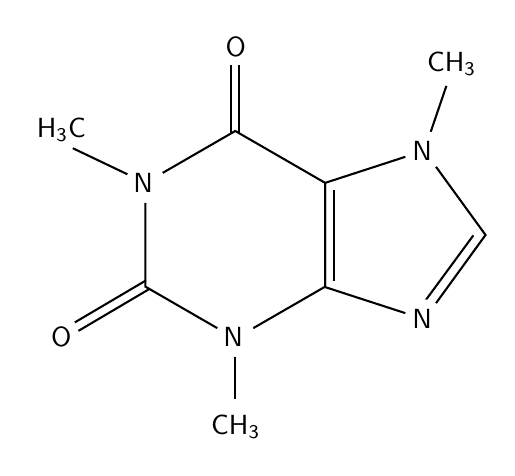
\begin{tikzpicture}[x=0.75pt,y=0.75pt,yscale=-1,xscale=1]
%uncomment if require: \path (0,300); %set diagram left start at 0, and has height of 300

%Shape: Regular Polygon [id:dp004400094577923452]
\draw   (231.6,166.7) -- (188.3,191.7) -- (145,166.7) -- (145,116.7) -- (188.3,91.7) -- (231.6,116.7) -- cycle ;
%Shape: Regular Polygon [id:dp7925754861532168]
\draw   (308.87,141.8) -- (279.36,182.43) -- (231.6,166.91) -- (231.6,116.7) -- (279.36,101.18) -- cycle ;
%Straight Lines [id:da8473227113357105]
\draw    (236,120) -- (236,164) ;
%Straight Lines [id:da21728791560640182]
\draw    (303,142) -- (278,176) ;
%Straight Lines [id:da6777547908917203]
\draw    (145.26,163.7) -- (111,183.92) ;
%Straight Lines [id:da6898565491342596]
\draw    (186.3,60) -- (186.3,92.7) ;
%Shape: Boxed Line [id:dp47917299330626917]
\draw    (145,116.7) -- (110,100) ;
%Shape: Boxed Line [id:dp2519300628036698]
\draw    (279.36,101.18) -- (290,70) ;
%Straight Lines [id:da5432254903819835]
\draw    (188.3,190.9) -- (188.3,220.7) ;
%Straight Lines [id:da998950148390531]
\draw    (147,167.78) -- (112.74,188) ;
%Straight Lines [id:da7607342852654713]
\draw    (190.3,60) -- (190.3,92.7) ;

% Text Node
\draw  [draw opacity=0][fill={rgb, 255:red, 255; green, 255; blue, 255 }  ,fill opacity=1 ]  (145, 116.7) circle [x radius= 9.6, y radius= 9.6]   ;
\draw (145,116.7) node   [align=left] {\begin{minipage}[lt]{8.67pt}\setlength\topsep{0pt}
$\displaystyle \mathsf{N}$
\end{minipage}};
% Text Node
\draw  [draw opacity=0][fill={rgb, 255:red, 255; green, 255; blue, 255 }  ,fill opacity=1 ]  (188.3, 190.9) circle [x radius= 9.6, y radius= 9.6]   ;
\draw (188.3,190.9) node   [align=left] {\begin{minipage}[lt]{8.67pt}\setlength\topsep{0pt}
$\displaystyle \mathsf{N}$
\end{minipage}};
% Text Node
\draw  [draw opacity=0][fill={rgb, 255:red, 255; green, 255; blue, 255 }  ,fill opacity=1 ]  (279.36, 182.43) circle [x radius= 9.6, y radius= 9.6]   ;
\draw (279.36,182.43) node   [align=left] {\begin{minipage}[lt]{8.67pt}\setlength\topsep{0pt}
$\displaystyle \mathsf{N}$
\end{minipage}};
% Text Node
\draw  [draw opacity=0][fill={rgb, 255:red, 255; green, 255; blue, 255 }  ,fill opacity=1 ]  (279.36, 101.18) circle [x radius= 9.6, y radius= 9.6]   ;
\draw (279.36,101.18) node   [align=left] {\begin{minipage}[lt]{8.67pt}\setlength\topsep{0pt}
$\displaystyle \mathsf{N}$
\end{minipage}};
% Text Node
\draw (98.5,88) node   [align=left] {\begin{minipage}[lt]{8.67pt}\setlength\topsep{0pt}
\begin{center}
$\displaystyle \mathsf{H_{3} C}$
\end{center}

\end{minipage}};
% Text Node
\draw (182.5,231) node   [align=left] {\begin{minipage}[lt]{8.67pt}\setlength\topsep{0pt}
\begin{center}
$\displaystyle \mathsf{CH_{3}}$
\end{center}

\end{minipage}};
% Text Node
\draw (286.5,56) node   [align=left] {\begin{minipage}[lt]{8.67pt}\setlength\topsep{0pt}
\begin{center}
$\displaystyle \mathsf{CH_{3}}$
\end{center}

\end{minipage}};
% Text Node
\draw (188.5,51) node   [align=left] {\begin{minipage}[lt]{8.67pt}\setlength\topsep{0pt}
\begin{center}
$\displaystyle \mathsf{O}$
\end{center}

\end{minipage}};
% Text Node
\draw (104.5,191) node   [align=left] {\begin{minipage}[lt]{8.67pt}\setlength\topsep{0pt}
\begin{center}
$\displaystyle \mathsf{O}$
\end{center}

\end{minipage}};


\end{tikzpicture}